
\section{The robot Obrero}
\label{sec:platform}


\begin{figure}[tbp]
\centerline{
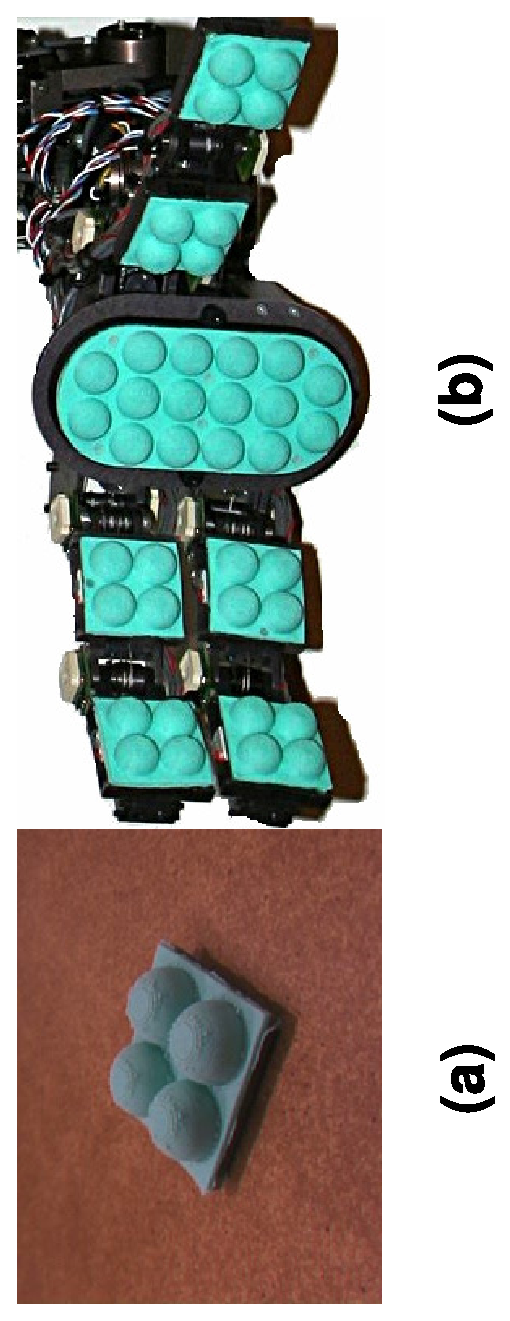
\includegraphics[width=1.0in, angle=270 ]{./figures/Tactiles.eps}
} \caption{Tactile Sensors. (a) Group of four tactile sensor. A
total of 16 sensors are read to determine the deformation of the
four tactile sensors. (b) Tactile sensors mounted on Obrero's
hand.} \label{fig:TactileSensors}
\end{figure}

Obrero \cite{obrero} consists of a hand, an arm and a head
(Figure~\ref{fig:RobotObrero}). Obrero was designed to approach
manipulation as a task manly guided by tactile and force feedback.
We use the robot's limb as a sensing/exploring device as opposed
to a pure acting device. This is a convenient approach to operate
in unstructured environments, on unmodeled objects. Obrero's limb
is sensor-rich and safe, it is designed to reduce the risk of
damages upon contact with objects. The head consists of a
commercial camcorder (SONY DCR-HC20) that can move along the pan
and tilt directions. The arm has 6 Degrees of Freedom (DOF)
distributed in this way: 3 in the shoulder, 1 at the level of the
elbow and 2 in the wrist. The arm mounts Series Elastic Actuators
\cite{williamson95series} which provide low-impedance and force
feedback at each joints (\cite{domo}). Position feedback is
provided by analog encoders (potentiometers).

The hand consists of a palm, a thumb, a middle and an
index finger. Each one of the fingers has two links that can be
opened and closed. The thumb and the middle finger can also
rotate. These rotations allow the the thumb to oppose to either
the index or the middle fingers.

%By rotating the thumb it can be opposed to the index
%finger and by rotating the thumb and the middle, they can oppose
%to each other.

The total number of degrees of freedom in the hand is 8. The hand
is underactuated, only 5 motors are connected to the fingers. Three motors control
the opening and closing of the fingers. The remaining two motors actuate
the rotation of the thumb and middle finger. The phalanges in each fingers
are mechanicaly coupled and actuated by a common motor. The link between
the two joints is realized by means of Series
Elastic Actuators, to allow independent motion
whenever one of the phalanges blocks (for example as a result of contact
with an object). This elastic coupling allows the hand to automatically
adapt to the object it grasps. All joints in the hand are equipped with an
optimized version of the Series Elastic Actuators \cite{actuator} which provide
force feedback and reduce the mechanical impedence of the fingers. Finally
position feedback is obtained through analog encoders mounted in all joints.

%However, they can decouple thanks to the SEA's in each
%joint. All the joints of the hand are controlled using an
%optimized design for a series elastic actuator \cite{actuator}.
%There are a total of 8 SEA's int the hand. Series elastic
%actuators\cite{williamson95series} reduce their mechanical
%impedance and provide force sensing.

The tactile sensors mounted on the robot were designed for robotic tasks.
Their design was inspired by the dome-like shape of the ridges that have been
observed in the human skin, where, the innervations at the base of the ridges
detect the deformation of the skin.

Inspired by this mechanism we realized a tactile sensor made of
silicon rubber and with a dome-like shape (see
figure\ref{fig:TactileSensors}a). At the tip of the dome, in the
internal part, we mounted a small magnet, whose position is
measured by four hall-effect sensors placed at the base. The
hall-effect sensors in this way measure the deformation of the
dome by sensing the position of the magnet at the tip. The sensors
are very sensitive and have been tested to detect up to the
minimum normal force of 10g.

The shape the sensors favors contact with the environment from any direction,
as opposed to most of the tactile sensors which are flat.
This high deformability and the properties of the silicon rubber allow the
sensors to conform to the objects, thus increasing friction and improving
contact detection.

In the particular implementation used in this paper, we used the
``magnetic'' version of the tactile sensors, however, a optical
version has been also tested. An analysis and description of the
design of these sensors can be found in \cite{etorresjSoft}.
Groups of tactile sensors were placed in parts of the hand. Two
groups of four were placed on each finger (a group in each of the
two phalanges) and 16 on the palm. A detail of the palm and
fingers can be observed in figure\ref{fig:TactileSensors}b . Each
one of these tactile sensors uses 4 sensors to determine the
contact forces. That means that overall the tactile feedback
consist of 160 sensors. At the base of the palm, where for
practical reasons, we were not able to mount these tactile
sensors, we placed a smaller infrared proximity sensor. To
summarize, the hand has 5 motors, 8 DOF, 8 force sensors, 10
position sensors, 160 tactile sensors and a infrared proximity
sensor.
